\documentclass{article}
\usepackage{hyperref}
\usepackage{amsmath,amssymb}
\usepackage{graphicx}
\usepackage{caption}
\usepackage{subcaption}
\usepackage[section]{placeins}
\renewcommand{\thesubsection}{\thesection.\alph{subsection}}

\title{\bf{CSE397: Assignment \#1}}
\author{Nicholas Malaya \\ Institute for Computational Engineering and Sciences \\ University of Texas at Austin} \date{}

\begin{document}
\maketitle

\newpage
\section{Problem 1}

\begin{figure}[!htb]
  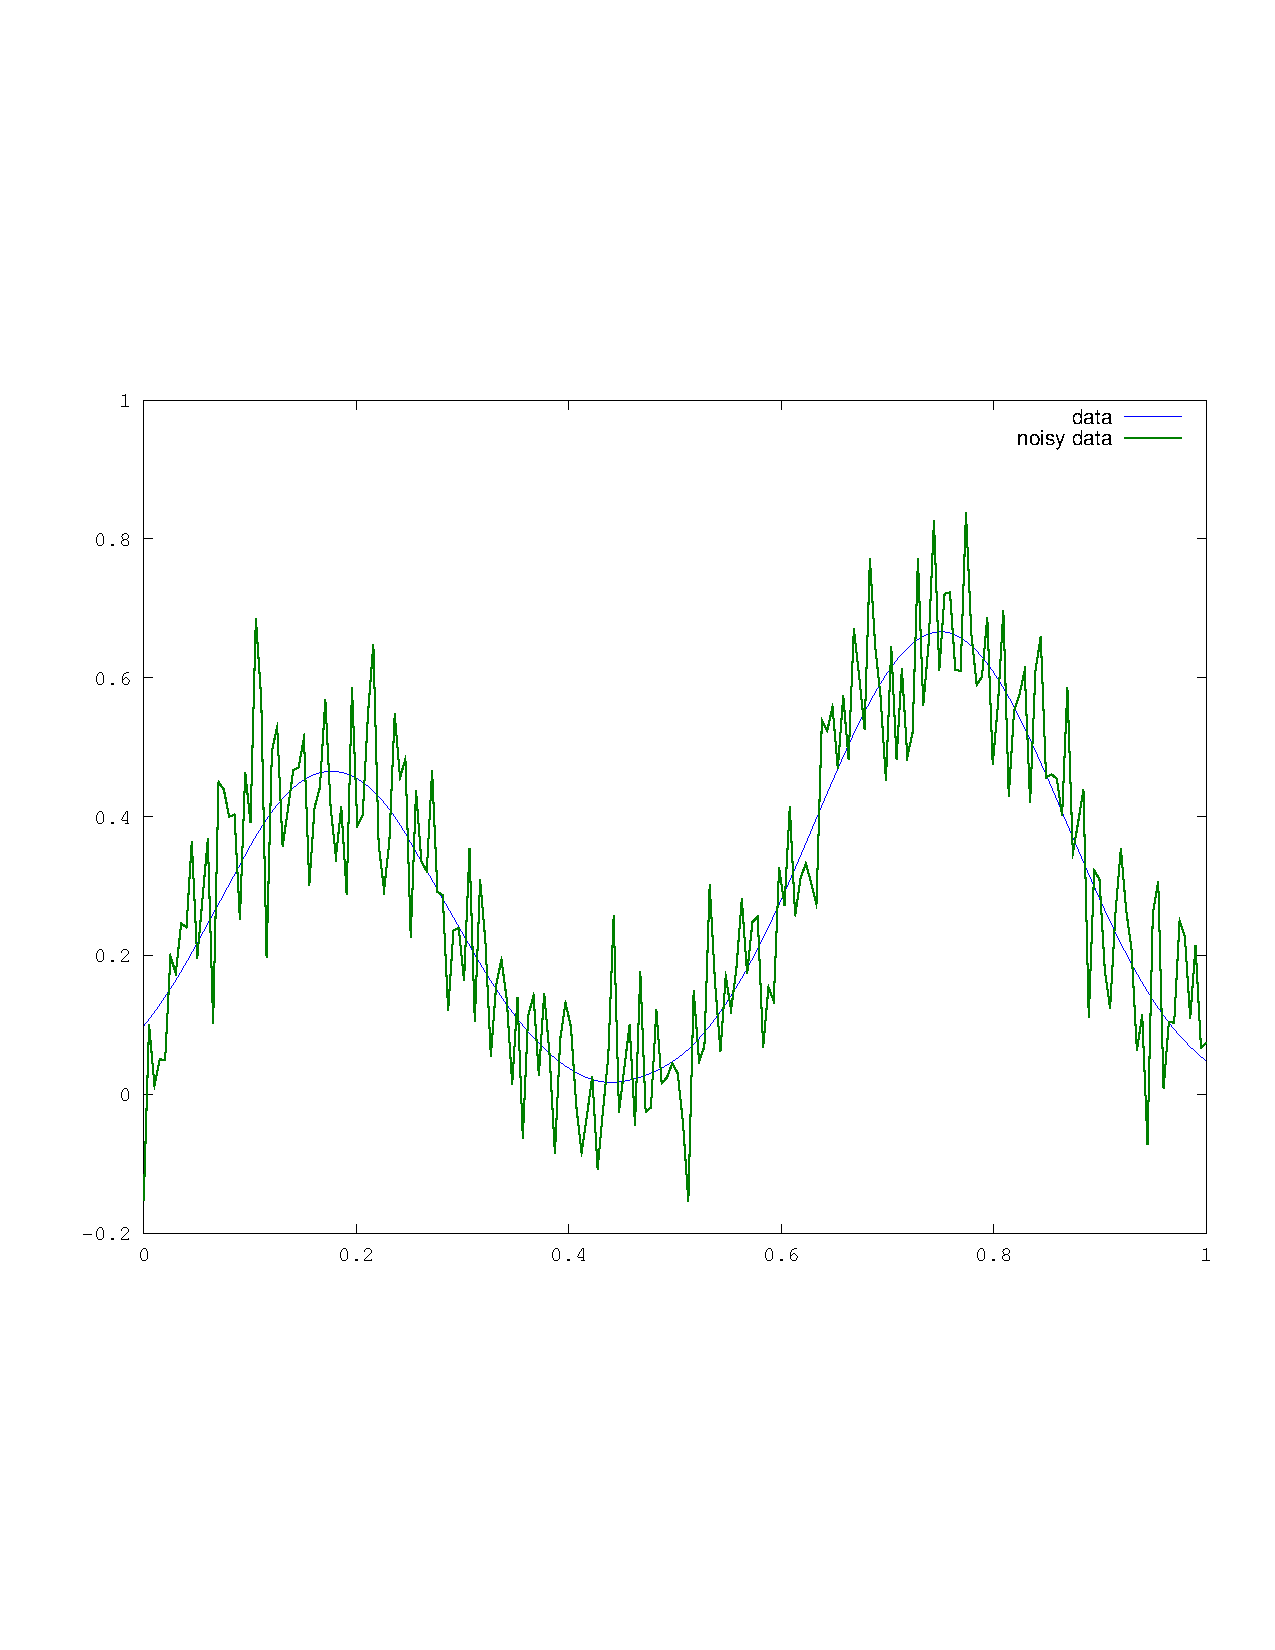
\includegraphics[scale=.5]{plots/data.pdf}
  \label{fig:data}
  \caption{The data (after applying the filter) with and without
 normally distributed noise. } 
\end{figure}

After applying the new filter $k(x)$ and adding gaussian noise, the data
used as input for the inverse problem is plotted in figure
\ref{fig:data}. 

Notice that this filter is significant: the raw data generated after
passing through the filter (even without statistical noise) has lost
several features of the underlying ``true'' signal. 

\subsection{$T_{\text{SVD}}$}


\begin{figure}[!htb]
        \centering
        \begin{subfigure}[bh]{0.45\textwidth}
                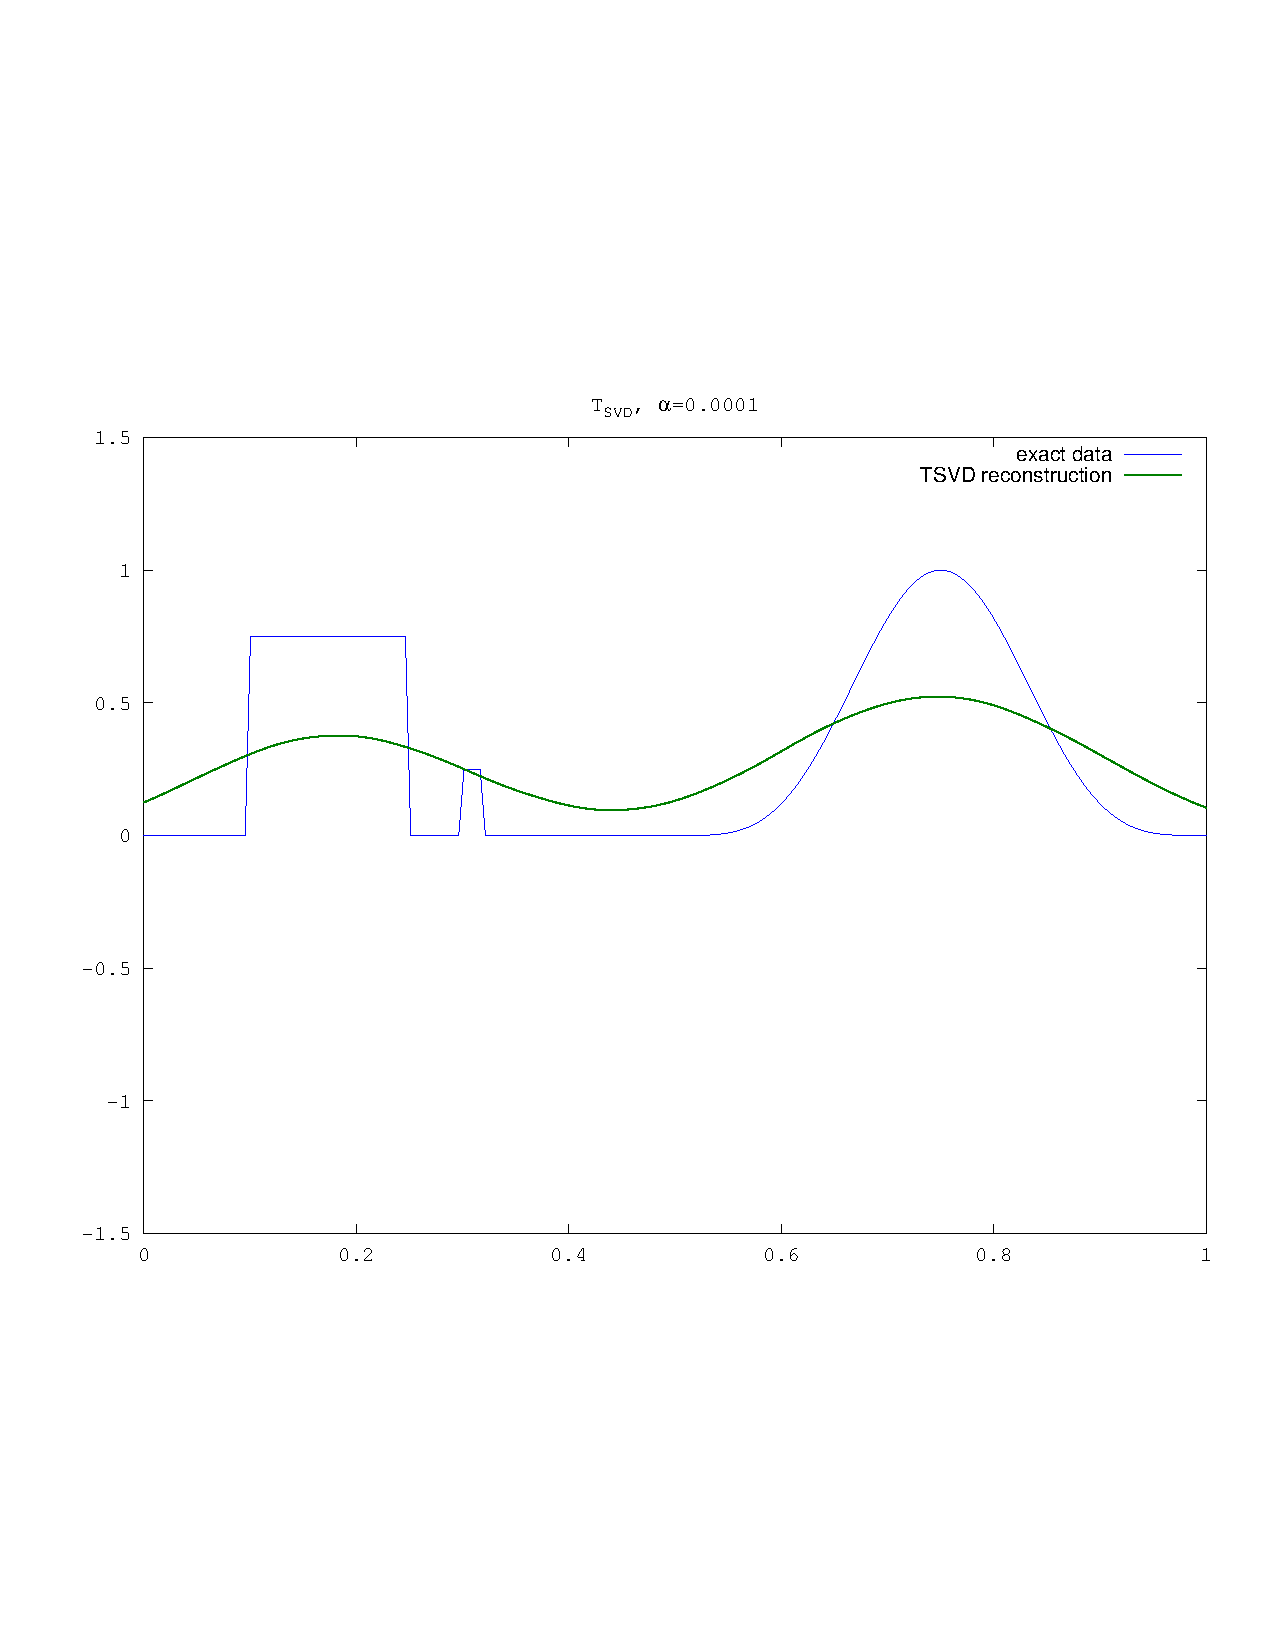
\includegraphics[width=\textwidth]{plots/tsvd0001.pdf}
                \caption{$\alpha=0.0001$}
        \end{subfigure}%
        \begin{subfigure}[bh]{0.45\textwidth}
                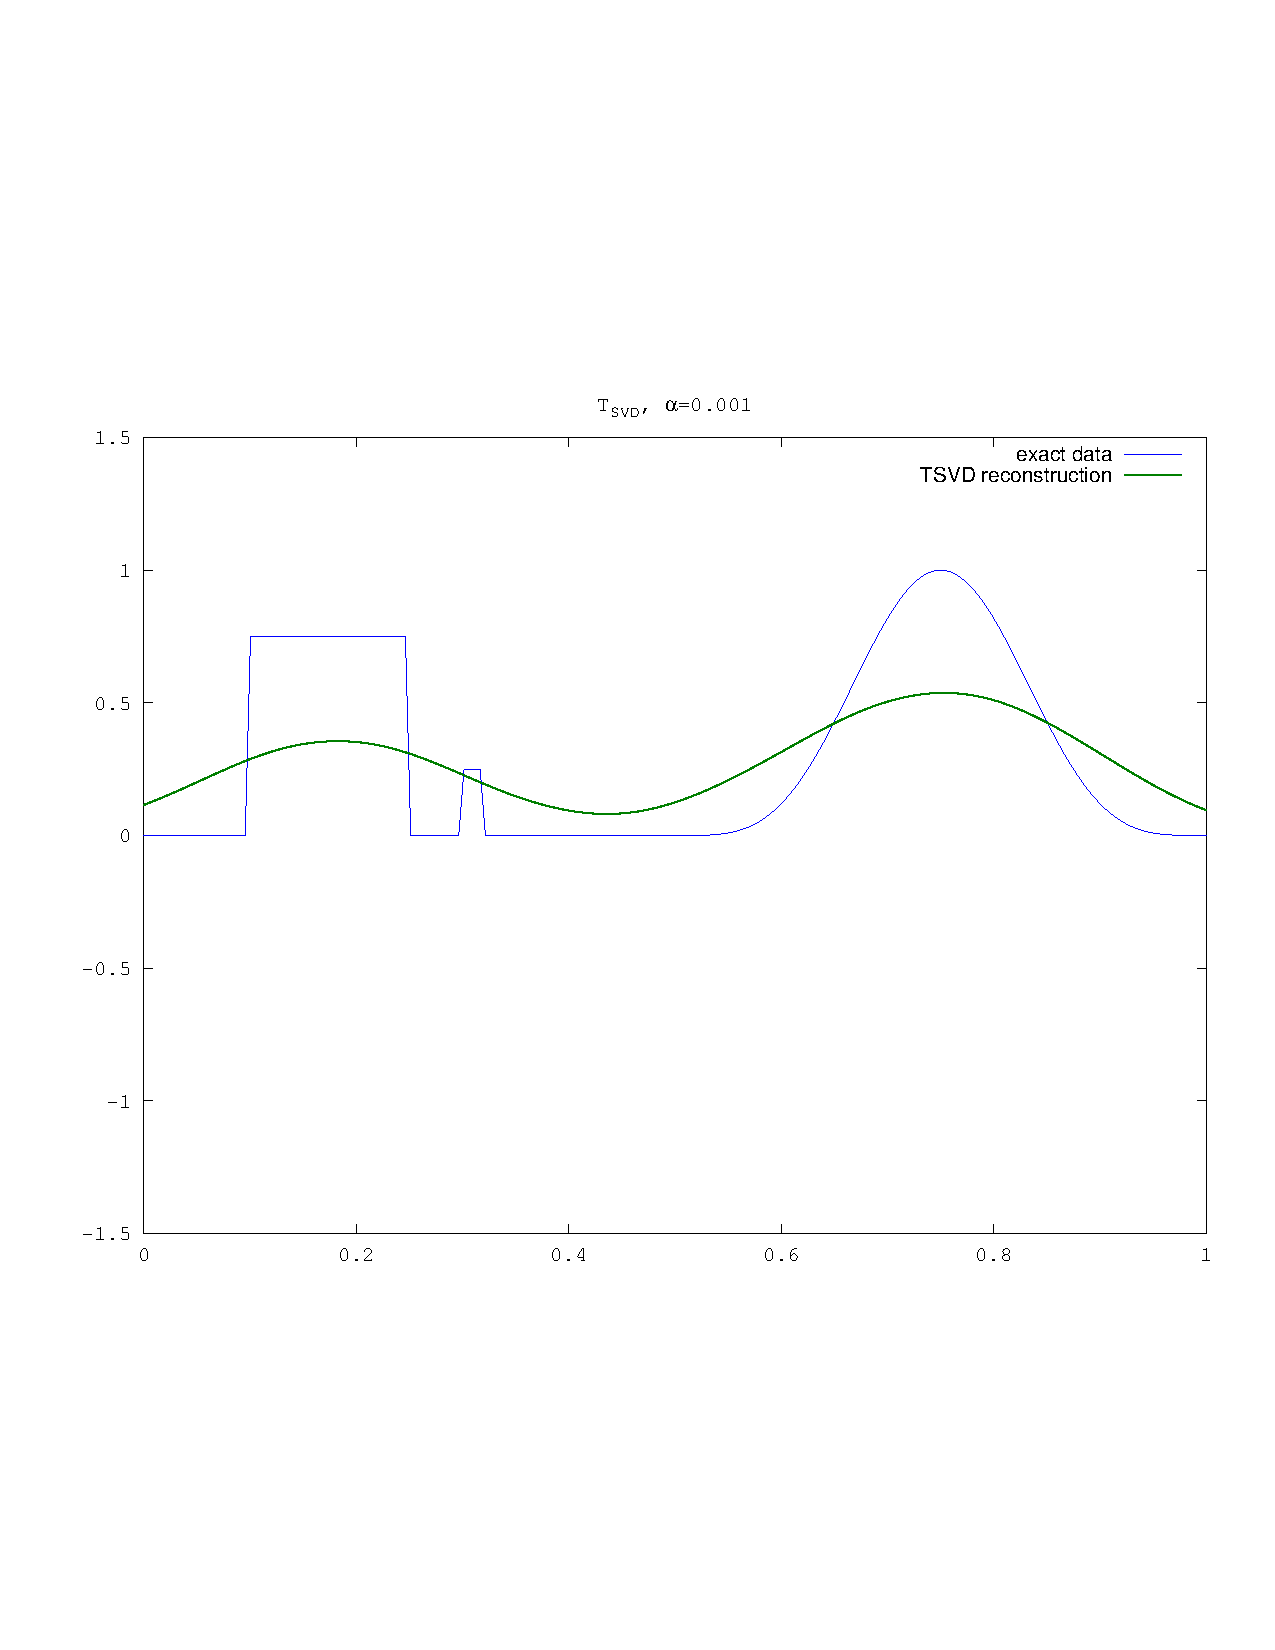
\includegraphics[width=\textwidth]{plots/tsvd001.pdf}
                \caption{$\alpha=0.001$}
        \end{subfigure}
        \centering
        \begin{subfigure}[bh]{0.45\textwidth}
                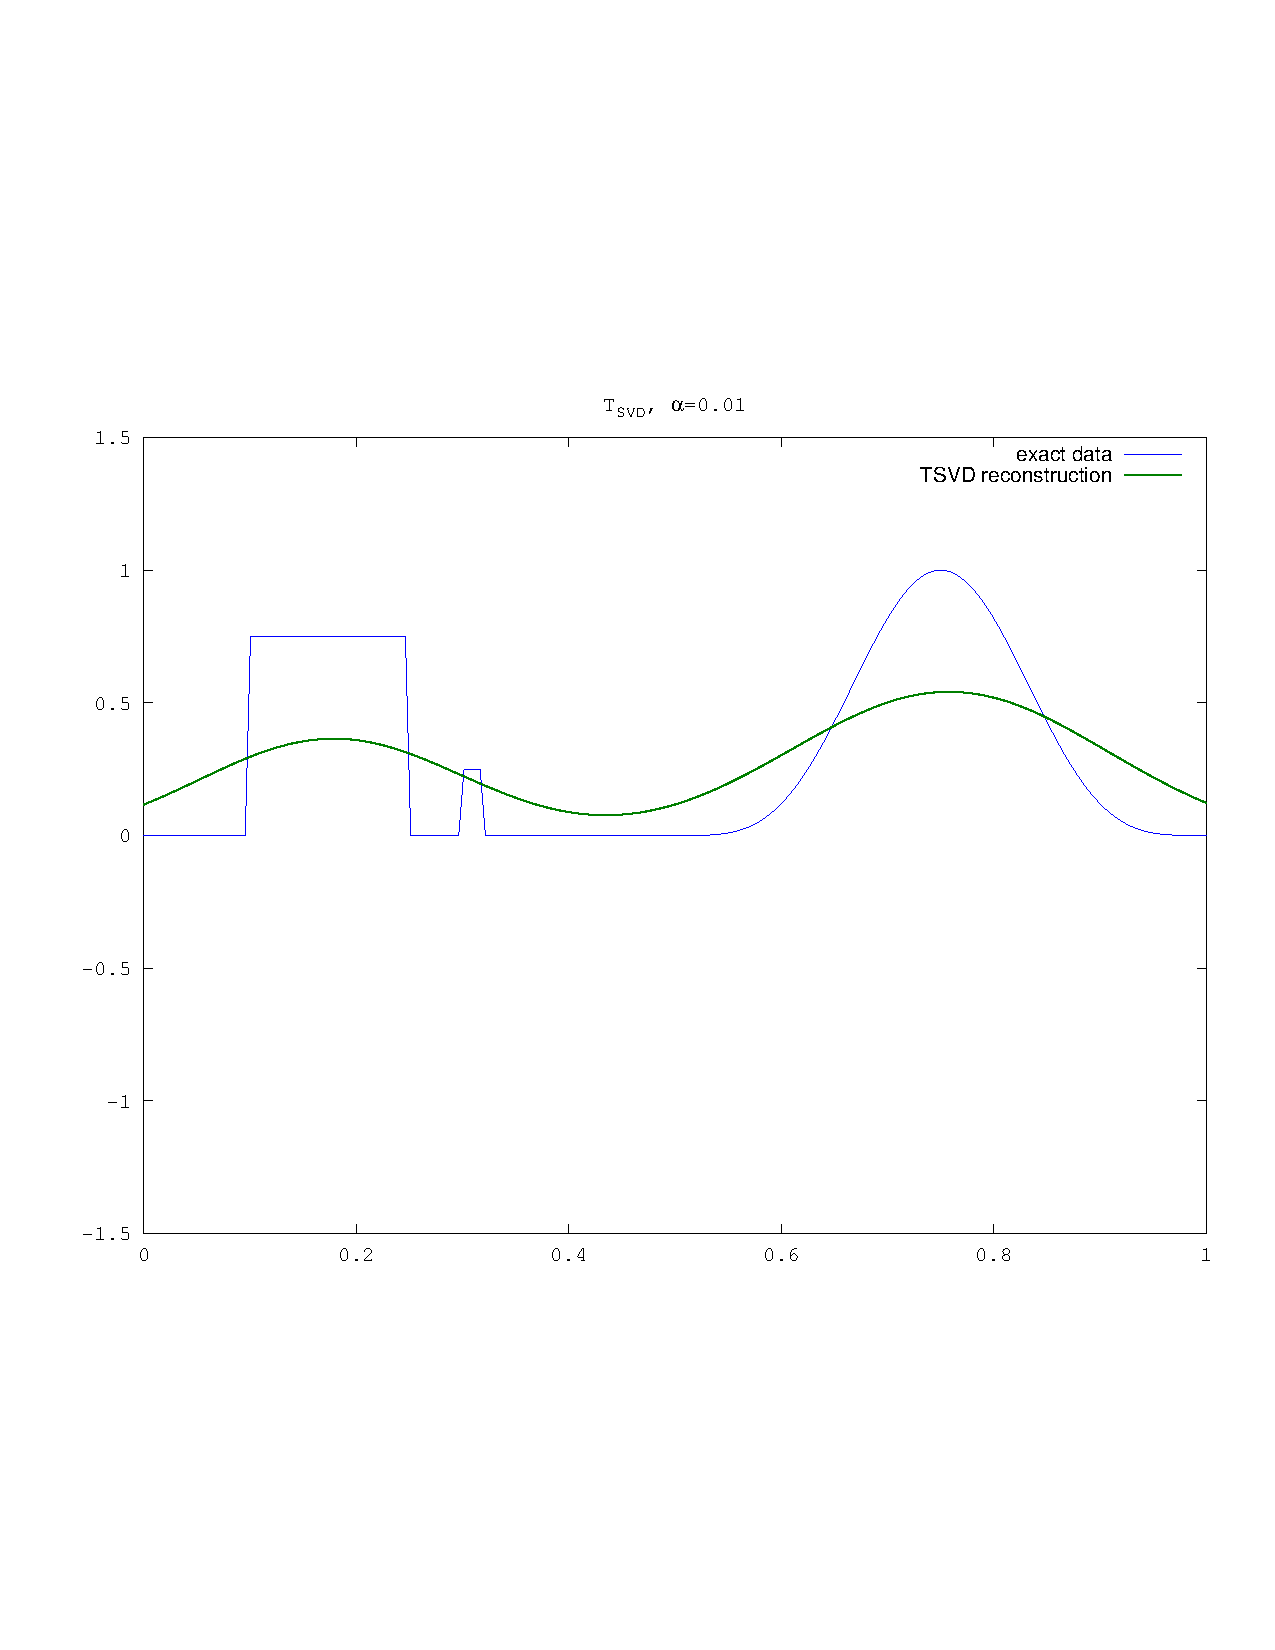
\includegraphics[width=\textwidth]{plots/tsvd01.pdf}
                \caption{$\alpha=0.1$}
        \end{subfigure}%
        \begin{subfigure}[bh]{0.45\textwidth}
                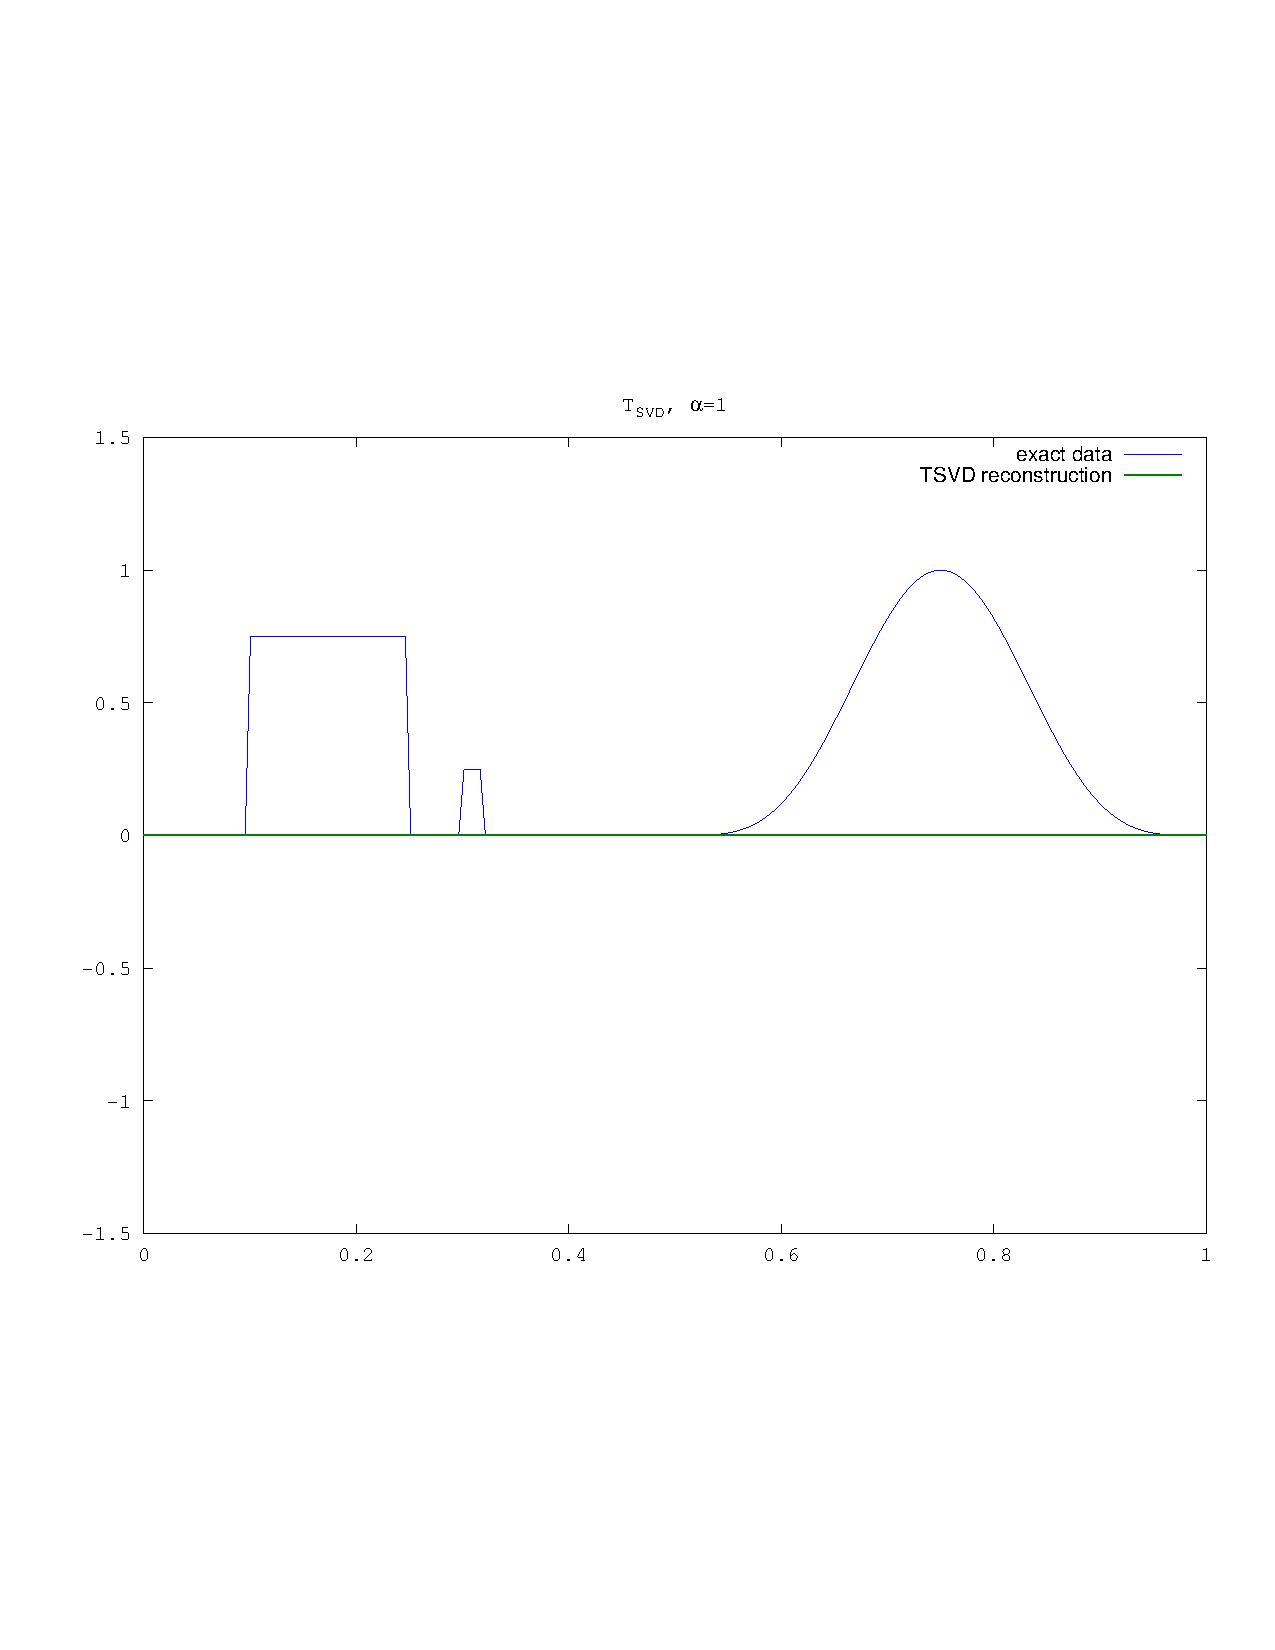
\includegraphics[width=\textwidth]{plots/tsvd1.pdf}
                \caption{$\alpha=1.0$}
        \end{subfigure}
        \caption{$T_{\text{SVD}}$ at varying values of $\alpha$.}
        \label{fig:svd}
\end{figure}

Figure \ref{fig:svd} plots the solution to the inverse problem using
Truncated SVD at several different values of
$\alpha$, the regularization parameter. 

\subsection{Tikhanov Filter}


\begin{figure}[!htb]
        \centering
        \begin{subfigure}[bh]{0.45\textwidth}
                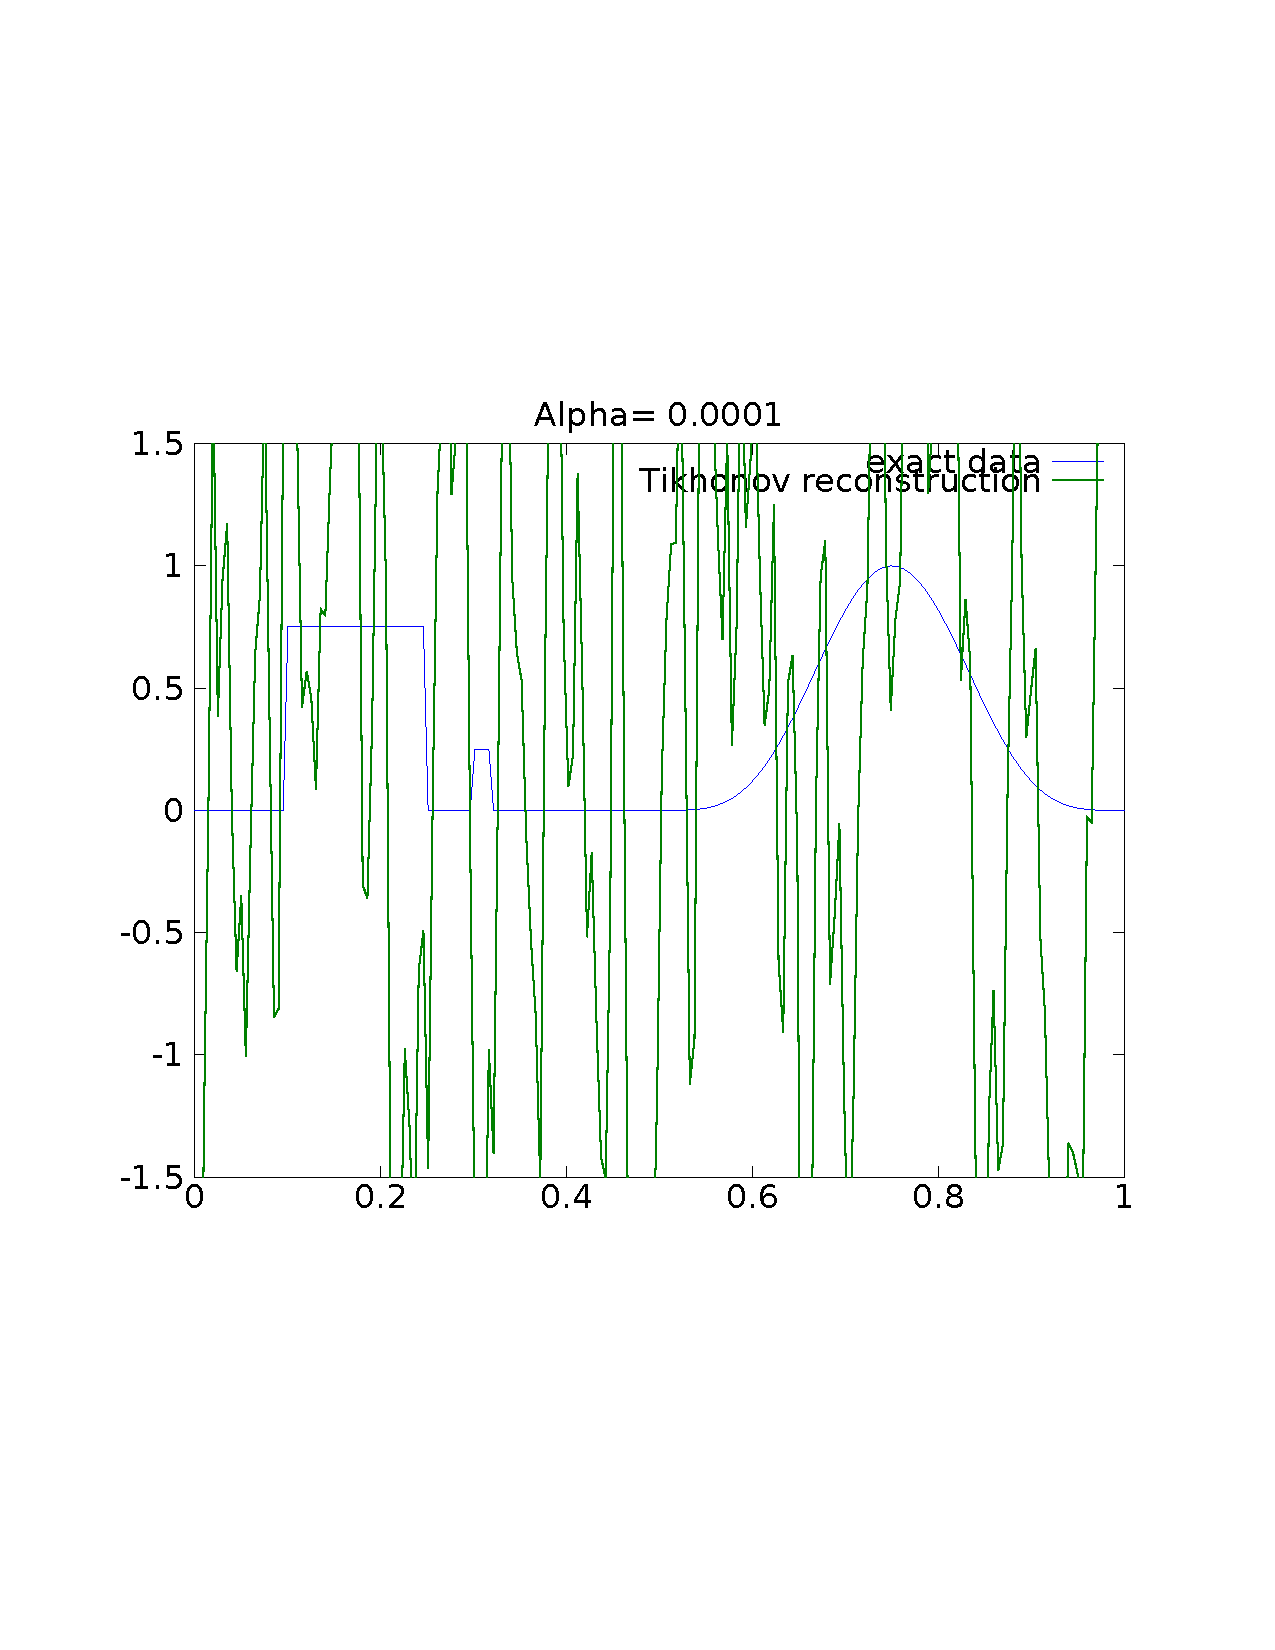
\includegraphics[width=\textwidth]{plots/reconstruct0001.pdf}
                \caption{$\alpha=0.0001$}
        \end{subfigure}%
        \begin{subfigure}[bh]{0.45\textwidth}
                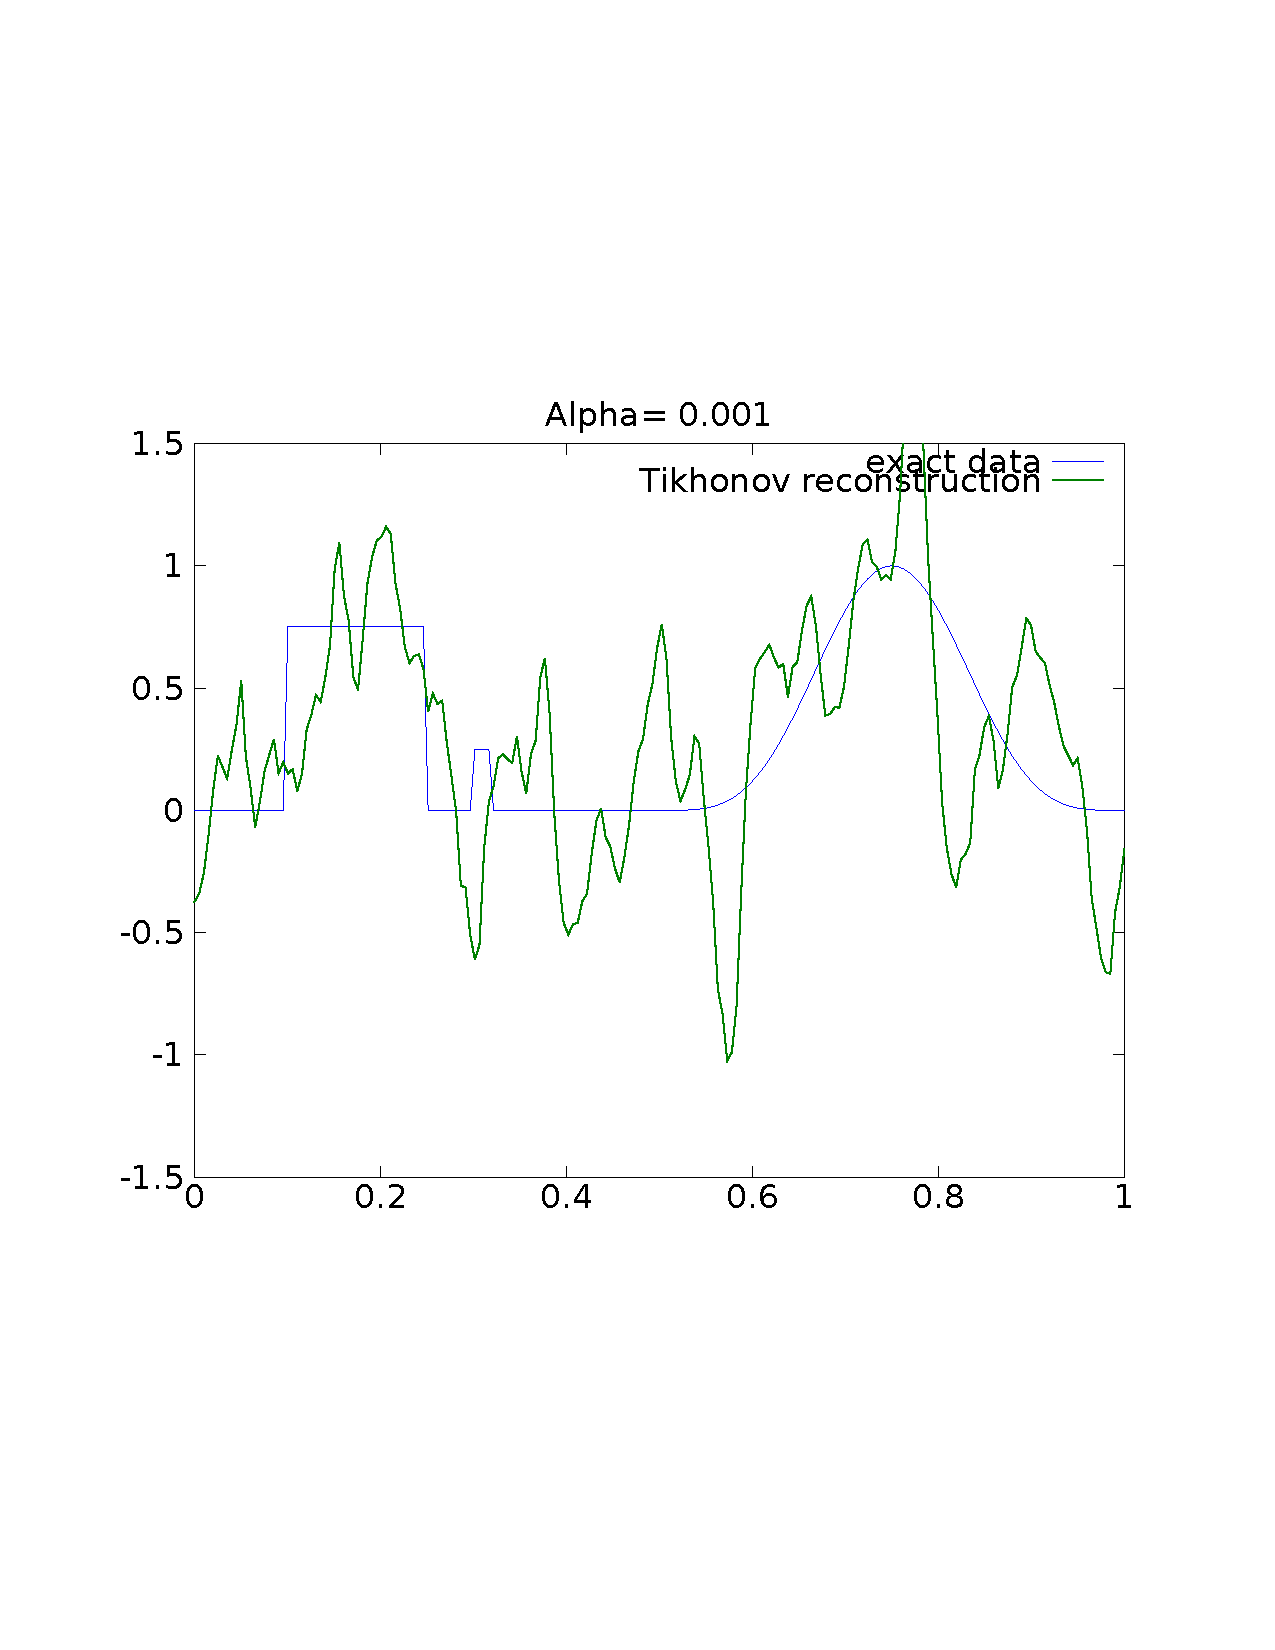
\includegraphics[width=\textwidth]{plots/reconstruct001.pdf}
                \caption{$\alpha=0.001$}
        \end{subfigure}
        \centering
        \begin{subfigure}[bh]{0.45\textwidth}
                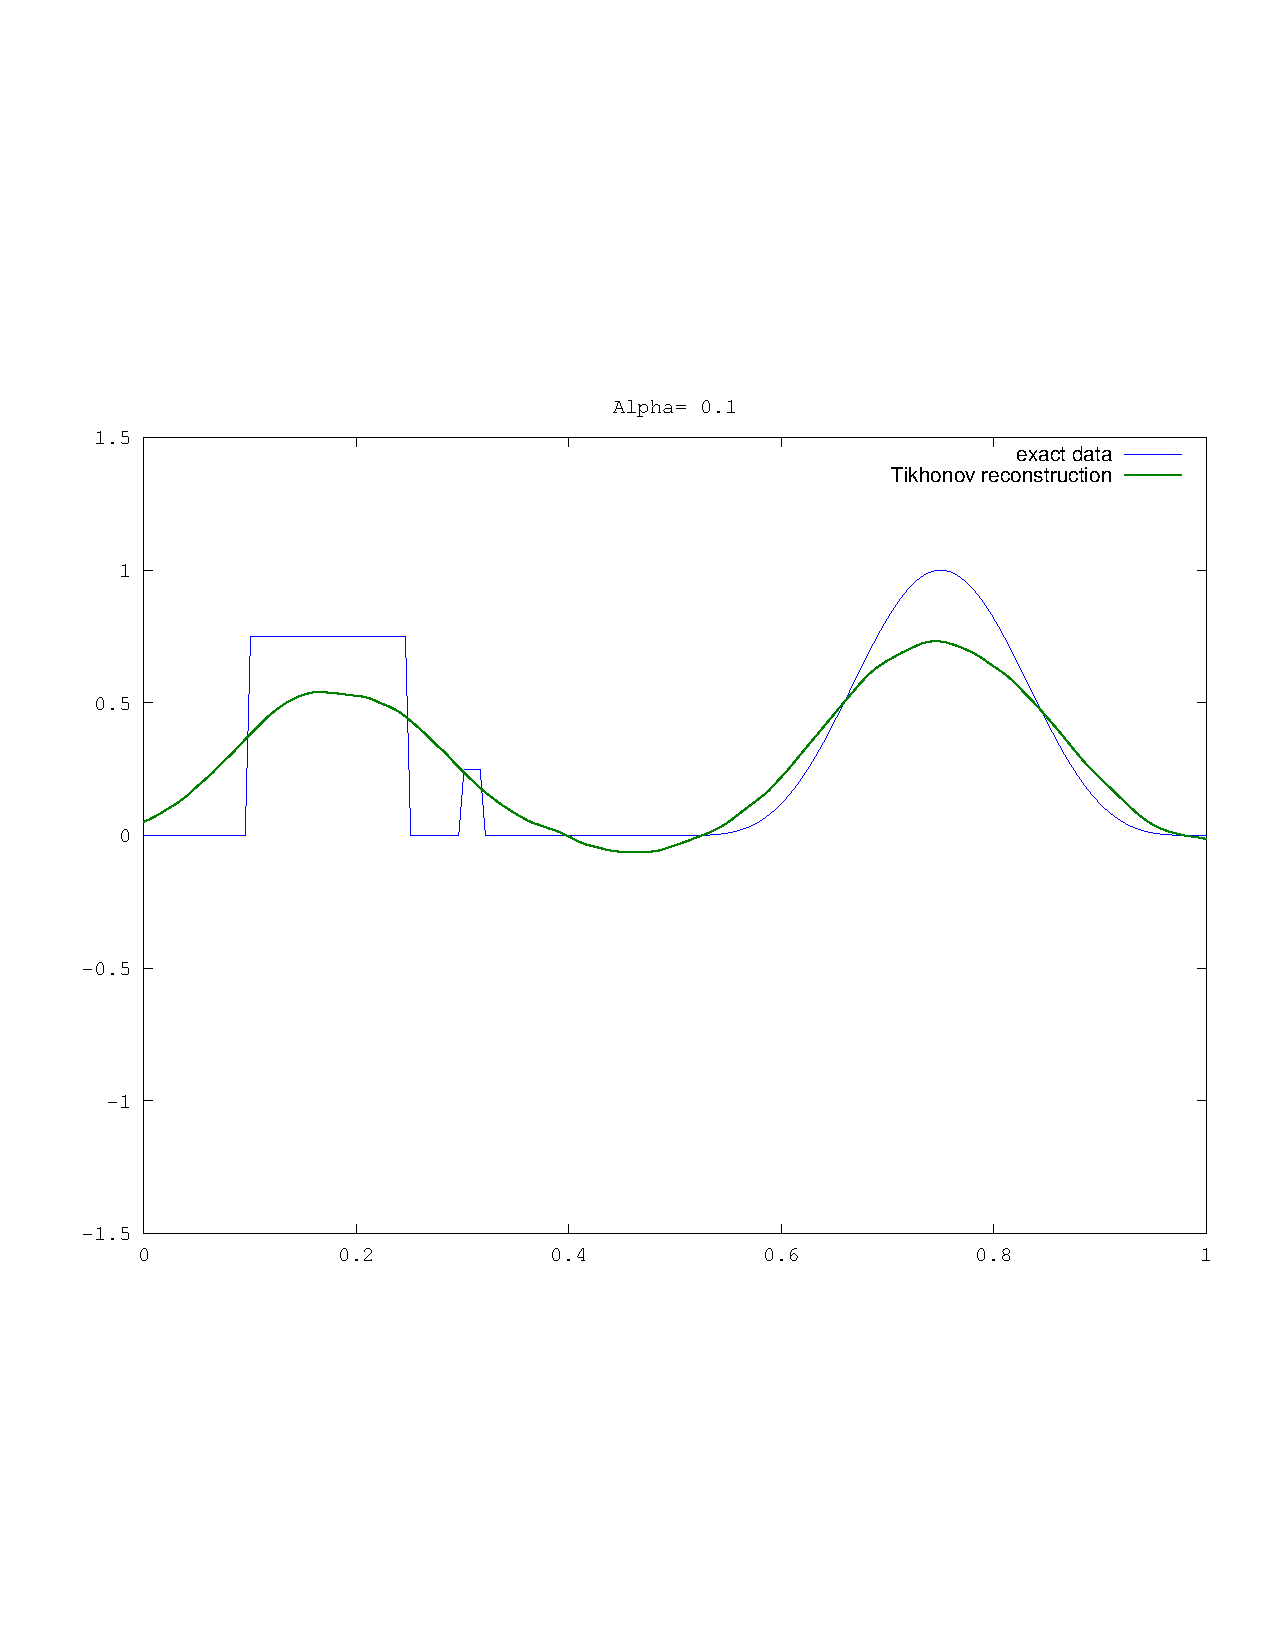
\includegraphics[width=\textwidth]{plots/reconstruct01.pdf}
                \caption{$\alpha=0.1$}
        \end{subfigure}%
        \begin{subfigure}[bh]{0.45\textwidth}
                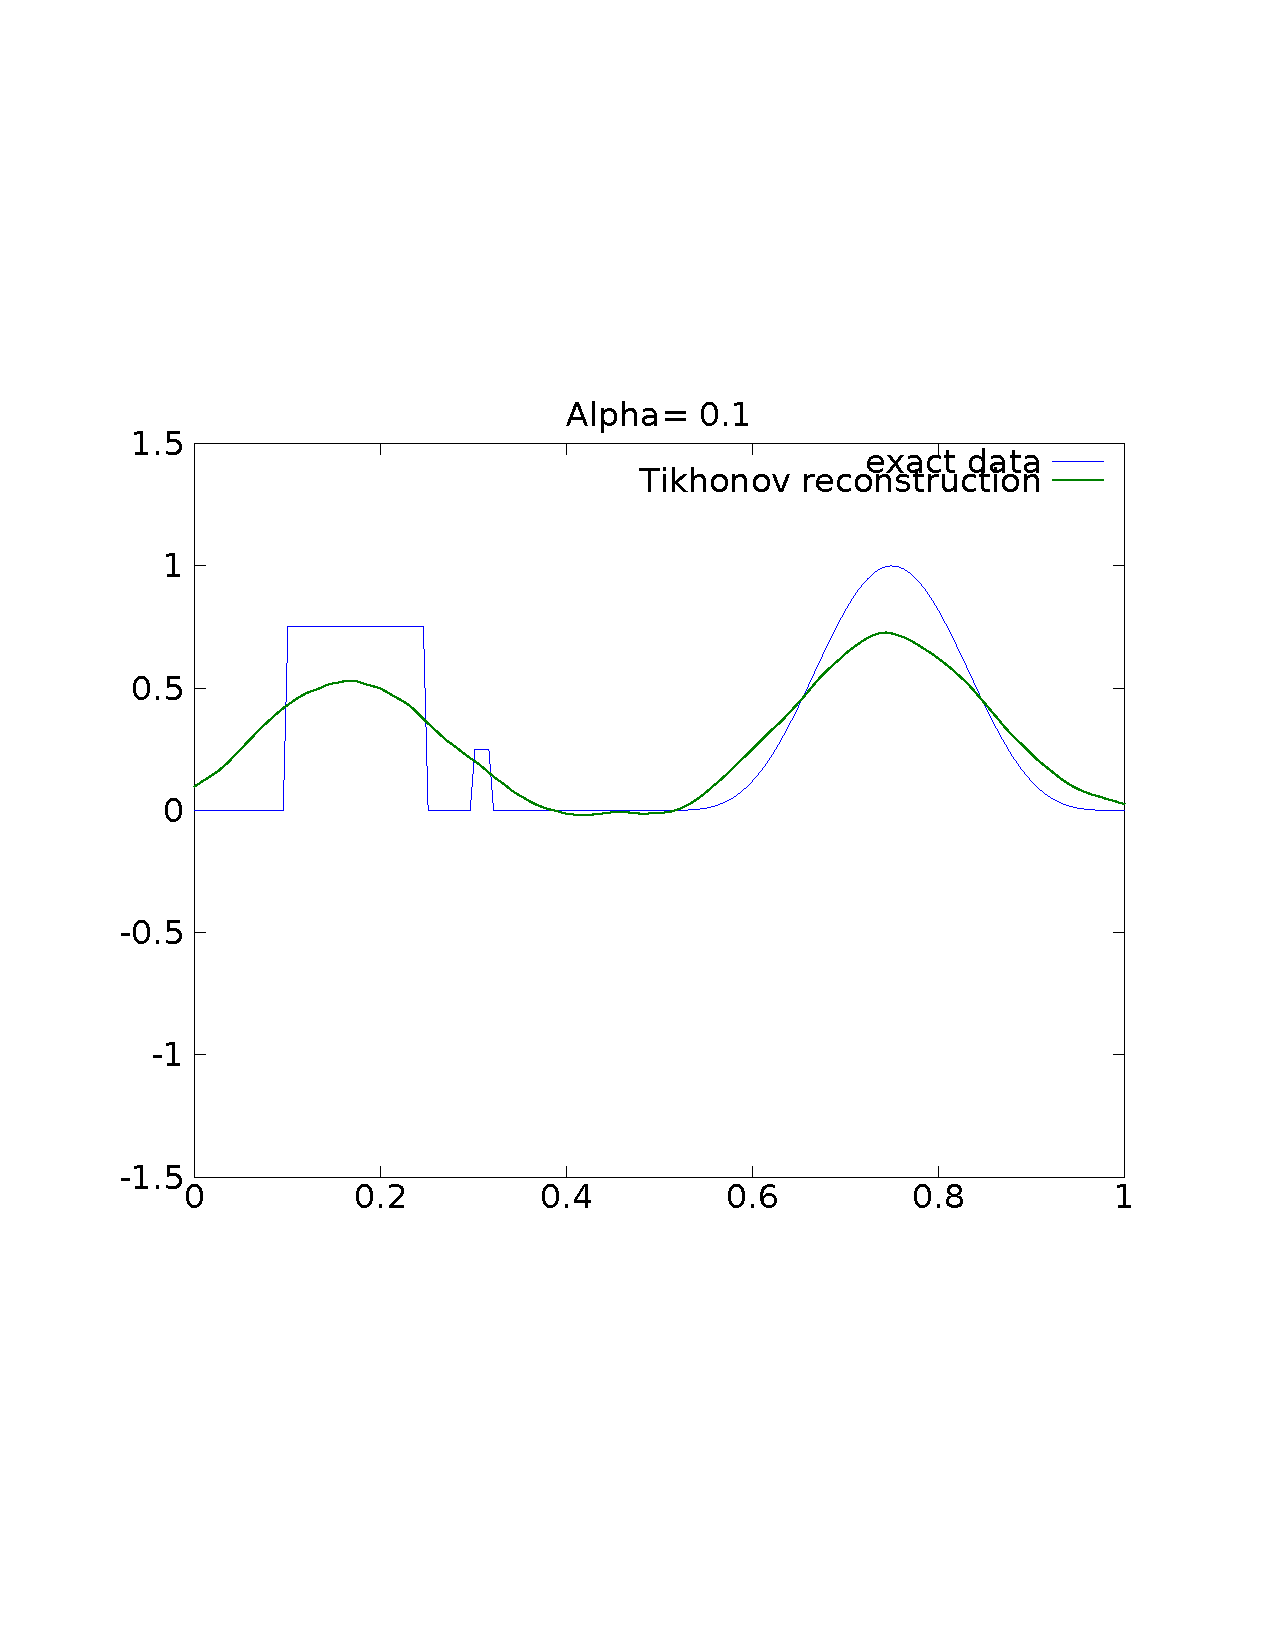
\includegraphics[width=\textwidth]{plots/reconstruct1.pdf}
                \caption{$\alpha=1.0$}
        \end{subfigure}
        \caption{Solutions to the inverse problem using Tikhanov
 regularization at varying values of $\alpha$.} 
 \label{fig:tik}
\end{figure}

Figure \ref{fig:tik} plots the solution to the inverse problem using
Tikhanov regularization at several different values of $\alpha$, the
regularization parameter.  

\subsection{L-Curve}

\begin{figure}[!htb]
  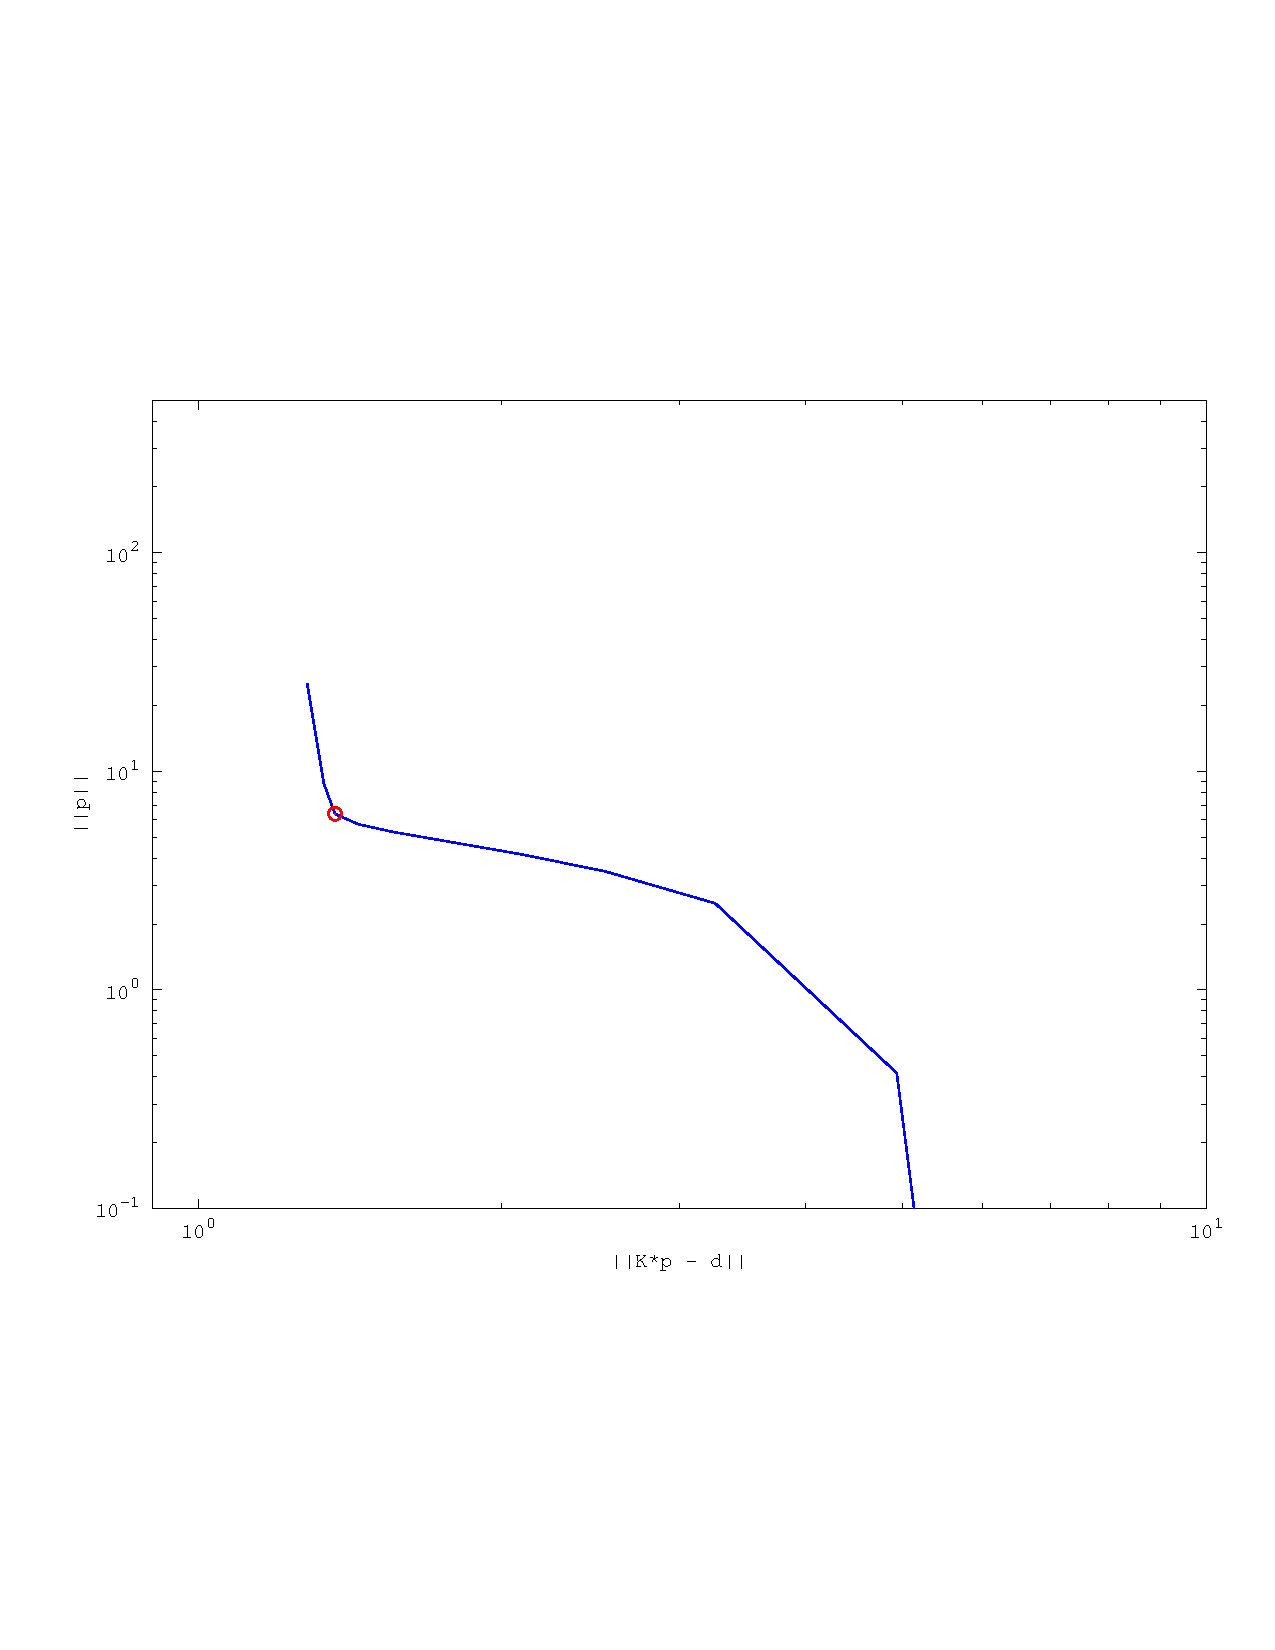
\includegraphics[scale=.5]{plots/L-curve.pdf}
  \label{fig:data}
  \caption{The L-curve} 
 \label{fig:lcurve}
\end{figure}

Figure \ref{fig:lcurve} plots the results of the L-curve criterion.


\subsection{Morozov's Discrepancy Criterion}

\begin{figure}[!htb]
  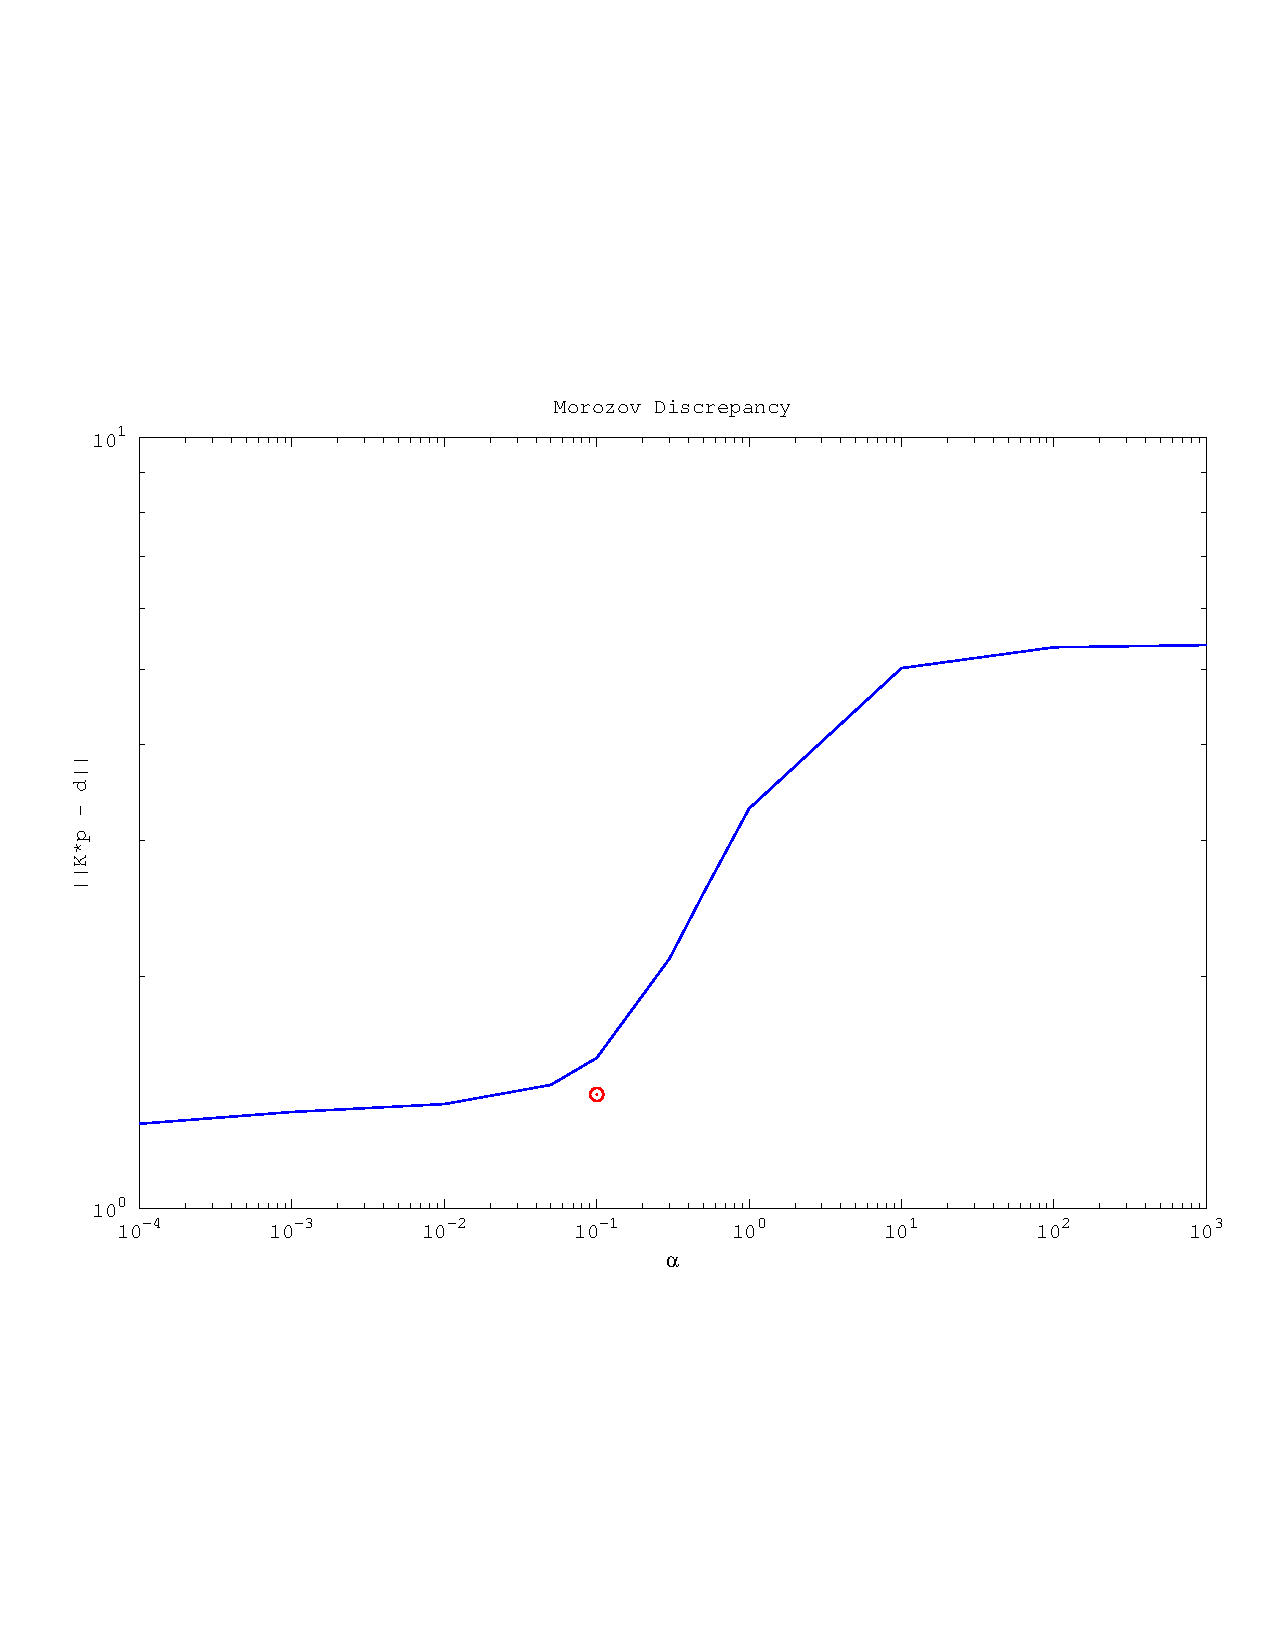
\includegraphics[scale=.5]{plots/morozov.pdf}
  \label{fig:data}
  \caption{Morozov discrepancy Criterion} 
 \label{fig:moro}
\end{figure}

Figure \ref{fig:moro} plots the results of Morozov discrepancy
criterion. I could not get the plots to draw a horizontal line, so that
red dot instead dictates the limit of $\delta$, the norm of the error. 


\subsection{Actual Error}

\begin{figure}[!htb]
  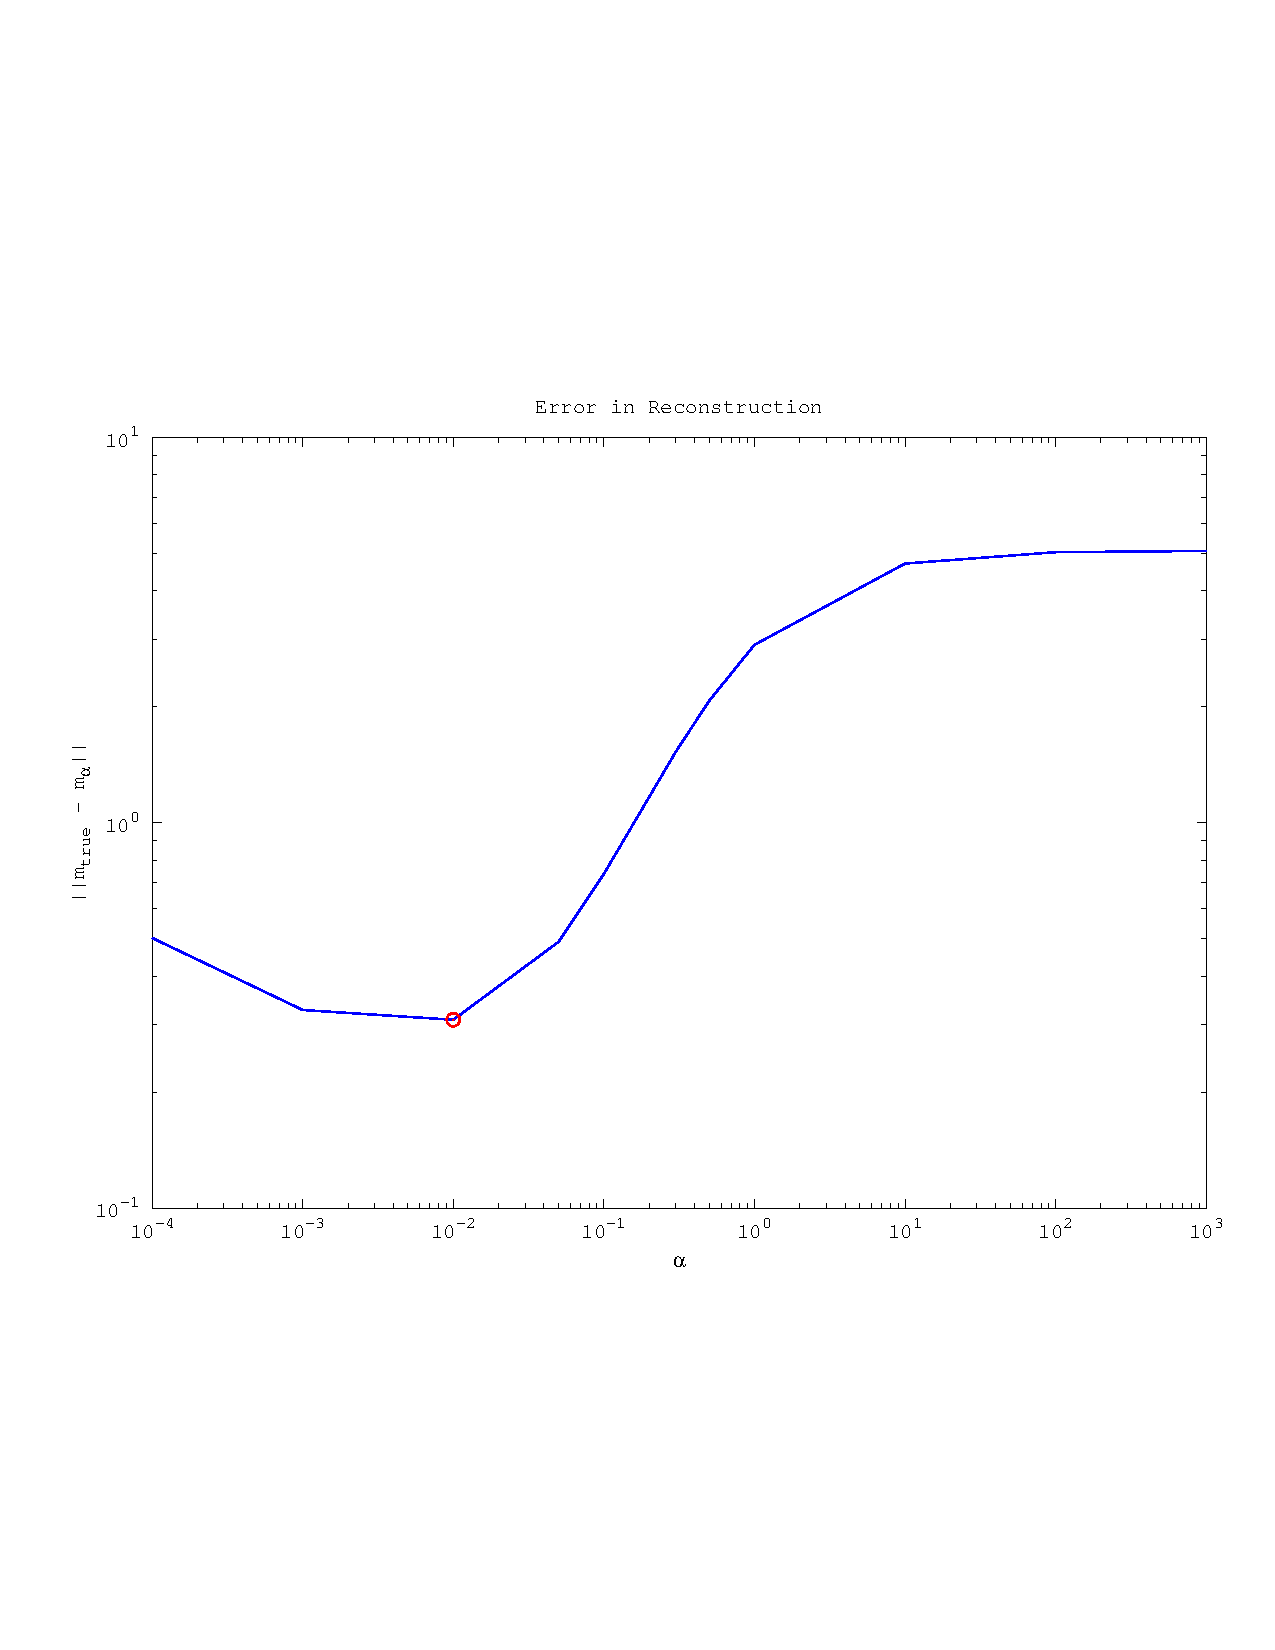
\includegraphics[scale=.5]{plots/true1d.pdf}
  \label{fig:data}
  \caption{The actual error in the reconstruction as a function of
 alpha. } 
 \label{fig:actual}
\end{figure}

Figure \ref{fig:actual} plots actual error in the reconstruction,
e.g. the norm of the difference between the reconstruction and the
actual (true) image, as a function of alpha. 


\newpage
\section{Problem 2}


\subsection{Memory Requirement}


\subsection{L-Curve}


\subsection{Actual Error}

\end{document}